
\section{Introduction}
The ZK-48 ignition (German "Zündkasten 48 Ausgänge") system was developed because of the lack of affordable  programmable firing systems. Therefore the goal was set for a low cost, yet reliable and robust device, that works in any condition. This document provides all information surrounding this project and anyone with basic knowledge in electronics should be able to rebuild it for them self. Although this should not be viewed as an instruction on how to build this device, the author hopes it will be useful to a pyrotechnic and or electronics enthusiast. The finished device is shown in \Cref{fig:complete_with_trig_and_mod} with the trigger on the right and one ignition module on the left.

\begin{figure}[!ht]
    \centering
    \includegraphics[width=15cm]{./Figures/complete_with_trig_and_mod.JPG}
    \caption{The resulting complete system with trigger and one ignition module.}
    \label{fig:complete_with_trig_and_mod}     
\end{figure}

\subsection{Legal Disclaimer}
\textbf{Please check your local laws before you decide on building a system such as this, by your self! Some countries may have laws prohibiting the construction of home-made ignition systems. So get informed! The author of this document does not endorse illegal activities nor can he be held responsible for any person's illegal activities. According to Austrian law, to which the author is subject, the construction and use of self-made ignition systems in the private and professional sphere, is not regulated! This is not legal advice, so do your own research!}\\

\noindent \textbf{In this document electronic ignitable matches are refereed to as \textit{Bridge wire detonators} or short \textit{detonators} just for readability purposes. But this does not mean actual detonators (also in English called \textit{blasting caps}) are used, as they contain high explosives which are not legal without license in Austria! The author refers to the in German called "A-Typ Brückenzünder"\footurl{https://de.wikipedia.org/wiki/Br\%C3\%BCckenz\%C3\%BCnder} which are legal to purchase by any person over 18 years of age. Again, this is not legal advise and do proper research on your local laws!}

\pagebreak
\subsection{Concept}
\label{Concept}
The device is divided into four units: controller,ignition voltage generator, trigger and ignition modules (See \Cref{fig:concept}), whereby the controller makes up the center piece. On board the controller are the main on/off key-switch, the arm switch,a USB port for programming, status LEDs and sockets for the trigger and ignition modules, as well as the micro controller (µC) which controls everything. The trigger is connected by cable to the controller and got mounted a arm switch and the trigger button for setting of the firework. There are six ignition modules and each module is able to ignite eight bridge wire detonators (A-Type Only). The modules are also connected by cable to the controller.  Therefore the complete system is capable of setting of 48 detonators.

\begin{figure}[!ht]
    \centering
    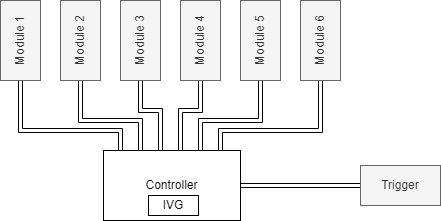
\includegraphics[width=10cm]{./Figures/concept_all.png}
    \caption{Basic layout of the three components controller, trigger and modules.}
    \label{fig:concept}     
\end{figure}

\noindent The system operates by the fire-and-forget principle, by which the user arms both the controller and the trigger and after pressing the trigger button the controller will automatically ignite the firework in the programmed sequence. No user input is needed after setting off. When the trigger is pressed the system goes into a $10s$ delay phase in order for the user to get to safety. After the delay phase is finished, the ignition phase is entered, where the programmed sequence will play through until the predetermined endpoint is reached. The trigger can be replaced with a RF-trigger although this is not recommend due safety and legal concerns in some countries. The delay period also serves as a fail safe, because in the case of an accidental triggering of the system, the user is able to abort the start by disarming the system. During the ignition phase it is also possible to halt the program by disarming the system, although re-triggering will repeat the delay phase.\\

\noindent The ignition sequence is programmed over USB (See \cref{USB Connection}). Programming the sequence can be accomplished by directly connecting to the serial port and typing the commands by hand or by using the Software provided(See \cref{Software}).\\

\noindent As the device is most likely to be placed in an open-air field, there is no way for it to be connected to mains power, therefore it has to be operated by batteries. However, the usage of rechargeable batteries such as LiPo-batteries was not desirable for this project, due cost issues and the additional requirement of protection circuits. A better alternative was found by using common $5V$ portable powerbanks for smart phones. Those already provide steady $5V$ with build-in protective mechanisms. Furthermore, nowadays many people use powerbanks and if the user forgets to charge or forgets the powerbank altogether, there is a high chance some will be able to provide one as replacement. A powerbank can be charged by a simple micro USB cable which is also very common and removes the need for a specialized charger.





\pagebreak